\section*{Problem 1 - Attitude Control of Satellite}
You can answer Problem 1 in this file/section. One subsection for each part of the problem might be a good solution. 

\subsection*{Problem 1.1} 
This is where you answer Problem 1.1. Equation (1) from the assignment can be written in \LaTeX{} as:
\begin{equation}
\label{eq:dynamics}		% The label is used when referring to this equation. 
	\begin{aligned}
		\dot{\mathbf{q}} = \mathbf{T}_q (\mathbf{q} ) \boldsymbol{\omega} \\
		\mathbf{I}_{CG} \dot{\boldsymbol{\omega}} - \mathbf{S} (\mathbf{I}_{CG} \boldsymbol{\omega} ) \boldsymbol{\omega} & =  \boldsymbol{\tau}
	\end{aligned}	
\end{equation}
You can now refer to this equation as \eqref{eq:dynamics} where the label ensures that the correct equation number is used. If you want to write an equation directly in the text (outside of the equation environment), use: $\dot{\mathbf{q}} = \mathbf{T}_q (\mathbf{q} ) \boldsymbol{\omega}$. % You have to use the dollar sign to write math symbols within a text. 

A matrix (and an equation without equation number) can be created as: 
\begin{equation*}	% The star indicates that you don't want to give this equation a number. Normally used if you don't refer to the equation.
	\mathbf{A} = 
	\begin{bmatrix}
		a & b & c \\ d & e & f \\ g & h & i
	\end{bmatrix} \quad
	\mathbf{B} = 
	\begin{bmatrix}
		a \\ b \\ c
	\end{bmatrix}
\end{equation*}

\subsection*{Problem 1.2}
Answer Problem 1.2 here. Bold words can be written as \textbf{something bold}. It is also possible to create a new section level:
\subsubsection*{Inner Section 1}
\emph{text..}

\subsubsection*{Inner Section 2}
...

\subsection*{Problem 1.3}
Answer Problem 1.3 here. Equation (2) from the assignment can be written as: 
\begin{equation}
  \label{eq:tau}
  \mathbf{\tau} = -\mathbf{K}_d \boldsymbol{\omega} - k_p \boldsymbol{\epsilon}
\end{equation}

\subsection*{Problem 1.4}
The quaternion error can be written as
 \begin{equation}
	 \tilde{\mathbf{q}} := \left[
	 \begin{array}{c}
		 \tilde{\eta} \\
		 \tilde{\epsilon}
	 \end{array}
	 \right] = \bar{\mathbf{q}}_d \otimes \mathbf{q} 
 \end{equation}

\subsection*{Problem 1.5}
In problems with simulations, you need to include figures in the report:
\begin{figure}[ht]
	\centering
	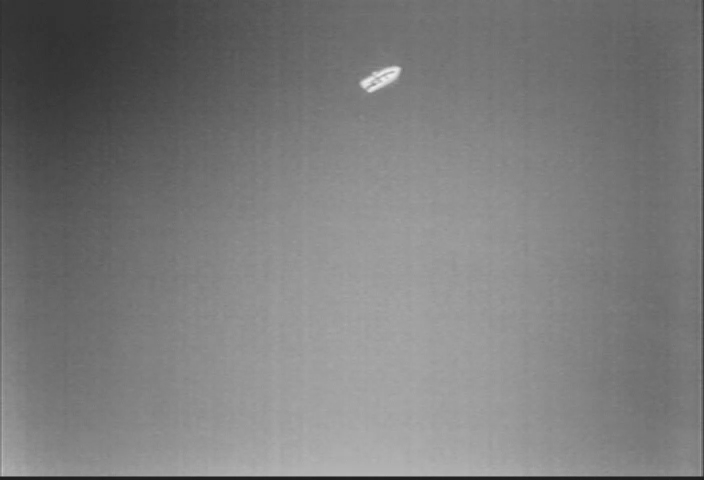
\includegraphics[width=0.7\textwidth]{fig1} % Filename is "fig1.png" and must be located in the same folder as this file. If you have a folder containing all the figures you can use "Figures/fig 1" as long as the "Figures" folder is placed in the same folder as this file.
	\caption{Figure of something useful.}
	\label{fig:fig1}
\end{figure}

You can now refer to this figure as \figref{fig:fig1}. You can also insert figures side-by-side as in Figure \ref{fig:2}. %Notice that \figref includes the word Figure before the reference. If you use "\ref", you need to write the word Figure yourself. 
\begin{figure}[ht]
	\centering
	\begin{subfigure}[b]{0.45\textwidth}
		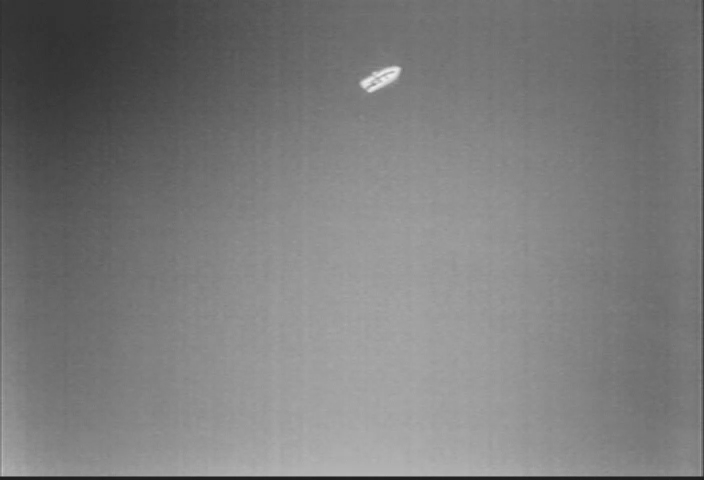
\includegraphics[width=\textwidth]{fig1}
		\caption{caption..}
		\label{fig:2a}
	\end{subfigure}
	~ %add desired spacing between images, e. g. ~, \quad, \qquad, \hfill etc. 
	%(or a blank line to force the subfigure onto a new line)
	\begin{subfigure}[b]{0.45\textwidth}
		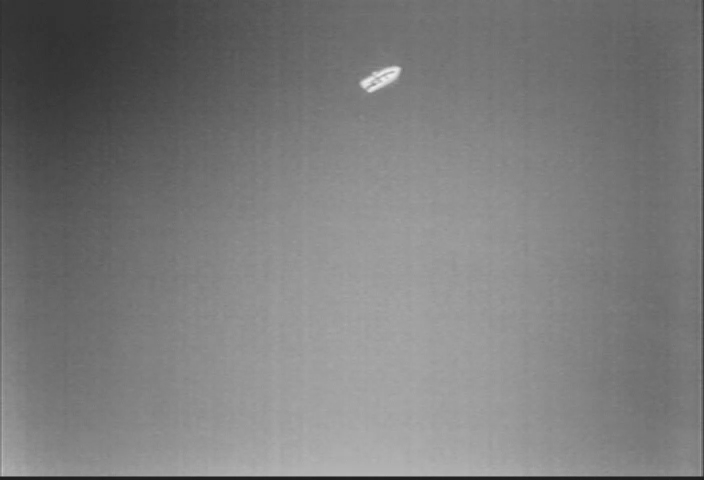
\includegraphics[width=\textwidth]{fig1}
		\caption{caption..}
		\label{fig:2b}
	\end{subfigure}
	\begin{subfigure}[b]{0.45\textwidth}
		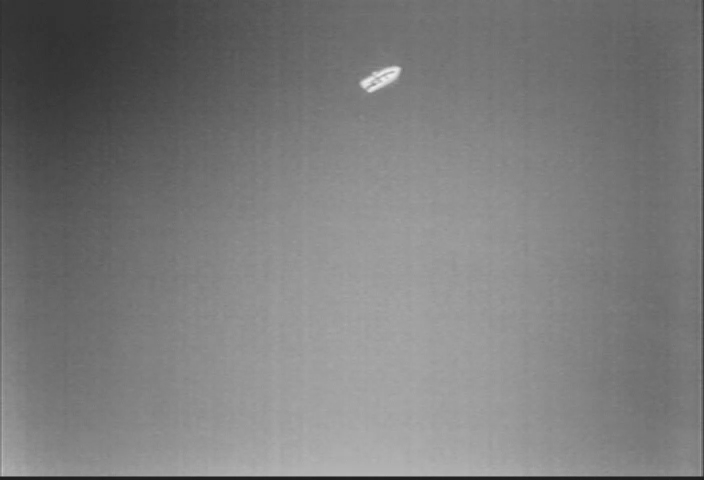
\includegraphics[width=\textwidth]{fig1}
		\caption{caption..}
		\label{fig:2c}
	\end{subfigure}
	\begin{subfigure}[b]{0.45\textwidth}
		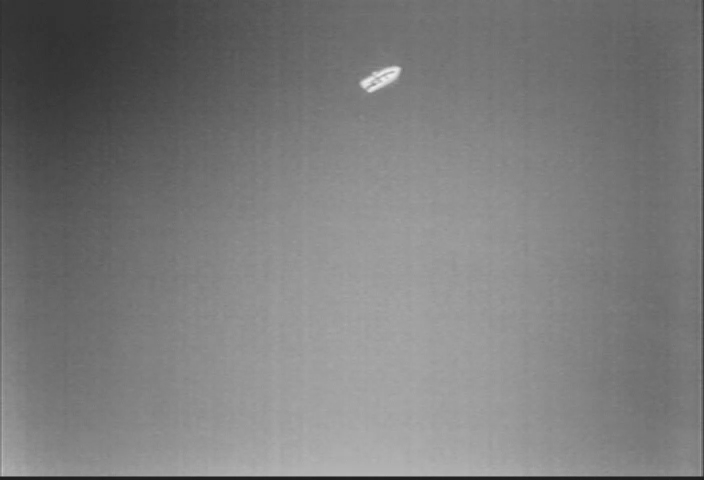
\includegraphics[width=\textwidth]{fig1}
		\caption{caption..}
		\label{fig:2d}
	\end{subfigure}		
	\caption{Caption for all figures}\label{fig:2}
\end{figure}


\subsection*{Problem 1.6}
The control law in this problem can be written as
\begin{equation}
	\boldsymbol{\tau} = -\mathbf{K}_d \tilde{\boldsymbol{\omega}} - k_p \tilde{\boldsymbol{\epsilon}}
\end{equation}
and the desired angular velocity as
\begin{equation}
	\boldsymbol{\omega}_d = \mathbf{T}^{-1}_{\Theta_d}(\Theta_d)\dot{\Theta}_d
\end{equation}

\subsection*{Problem 1.7}
The Lyapunov function can be written as 
 \begin{equation}
	 V = \frac{1}{2} \tilde{\boldsymbol{\omega}}^{\top} \mathbf{I}_{CG}\tilde{\boldsymbol{\omega}} + 2 k_p (1-\tilde{\eta})
 \end{equation}
and the derivative as 
\begin{equation}
	\dot{V} = -k_d \boldsymbol{\omega}^{\top} \boldsymbol{\omega}
\end{equation}

% Note that \mathbf can be used for bold letters in math mode (within equations and dollar signs). \boldsymbol can be used to get bold greek letters.  